\chapter{Anhang}
\section{ER-Modell}
\begin{figure}[ht]
	\centering
	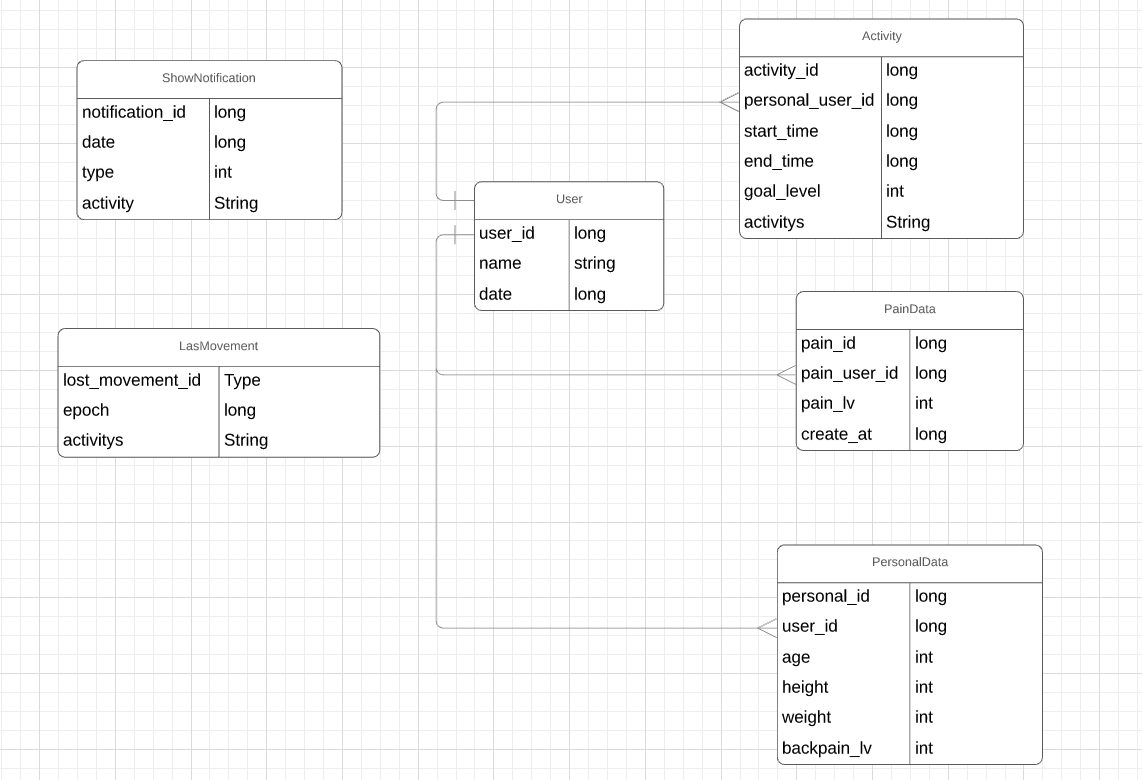
\includegraphics[width=1.1\textwidth]{Datenbank.png}
	\caption{\label{fig:ER-Modell}Grobes Datenbankmodell}
	
\end{figure}
\newpage

\section{Abbildungen}
\begin{figure}[ht]
	\centering
	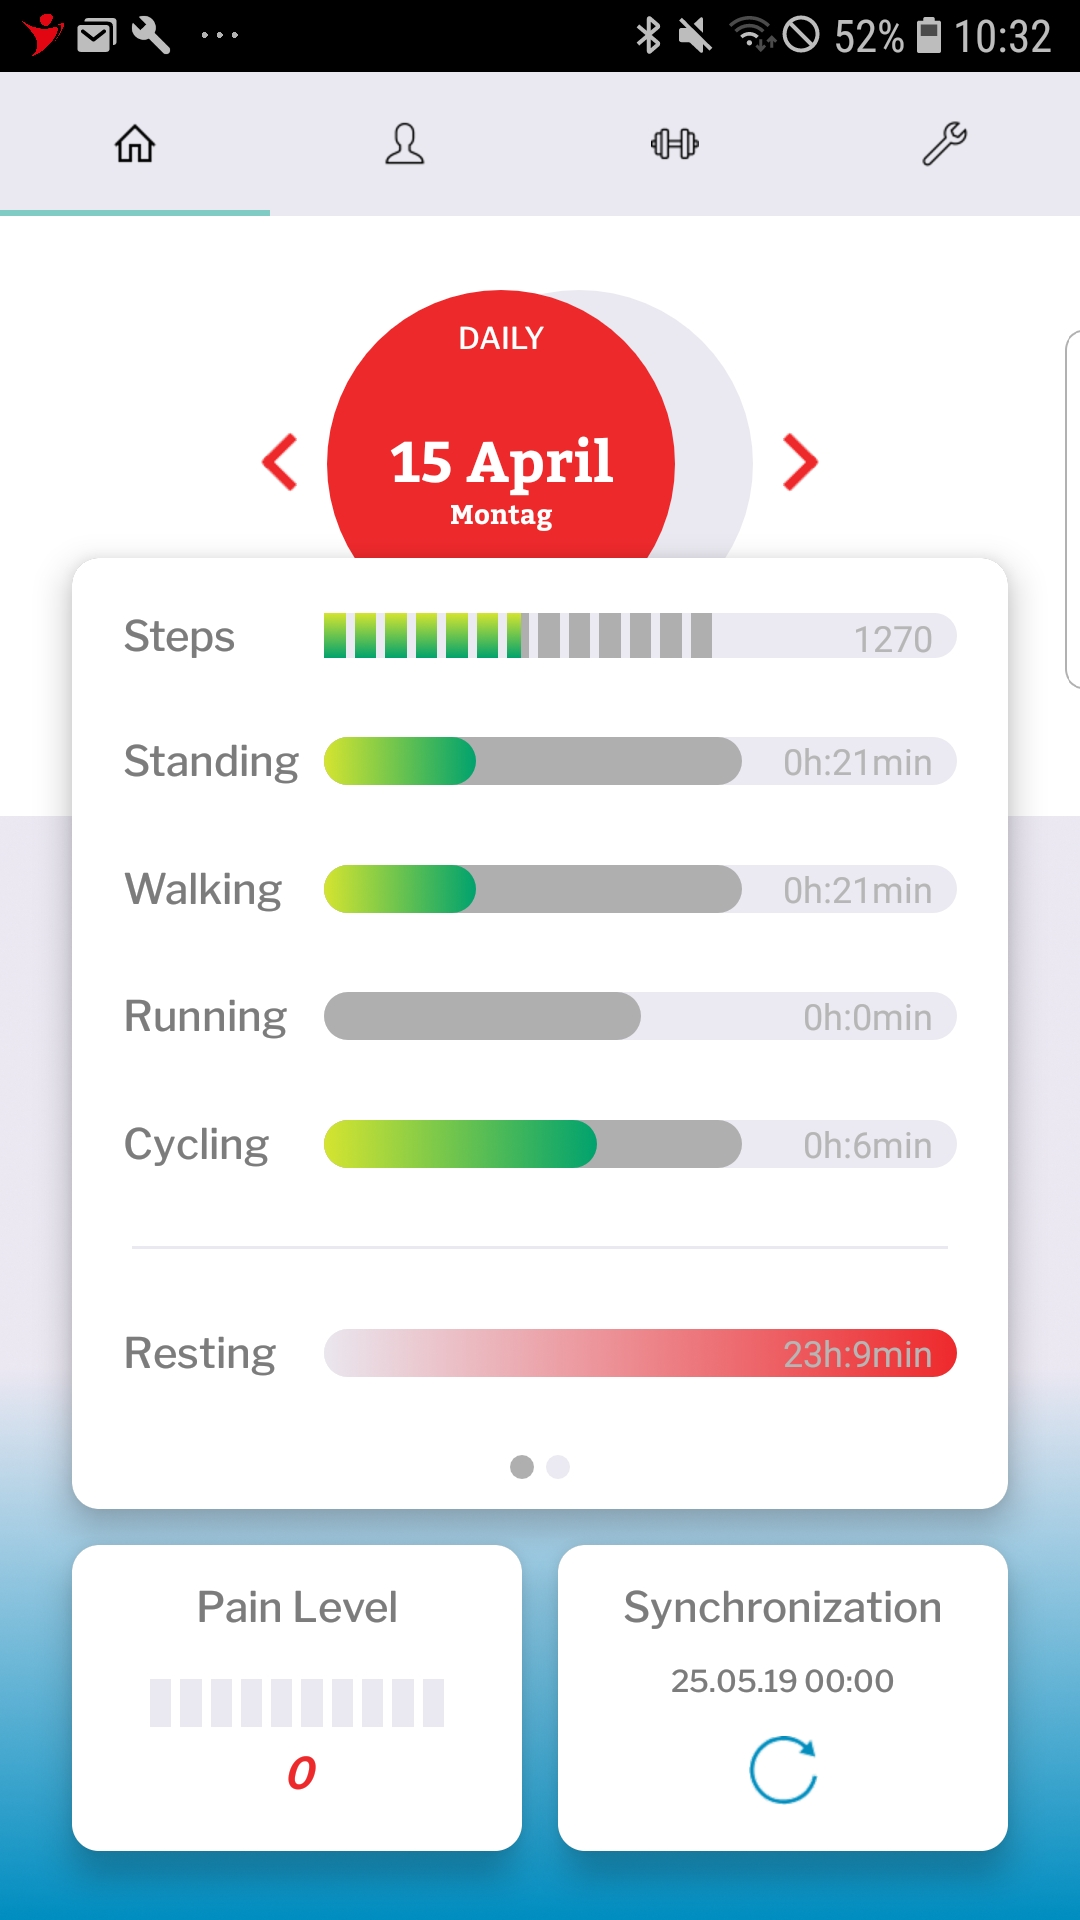
\includegraphics[width=0.5\textwidth]{Activitys.jpg}
	\caption{\label{fig:Activity}Aktivitäten mit den Daten von der API }
	
\end{figure}

\begin{figure}[ht]
	\centering
	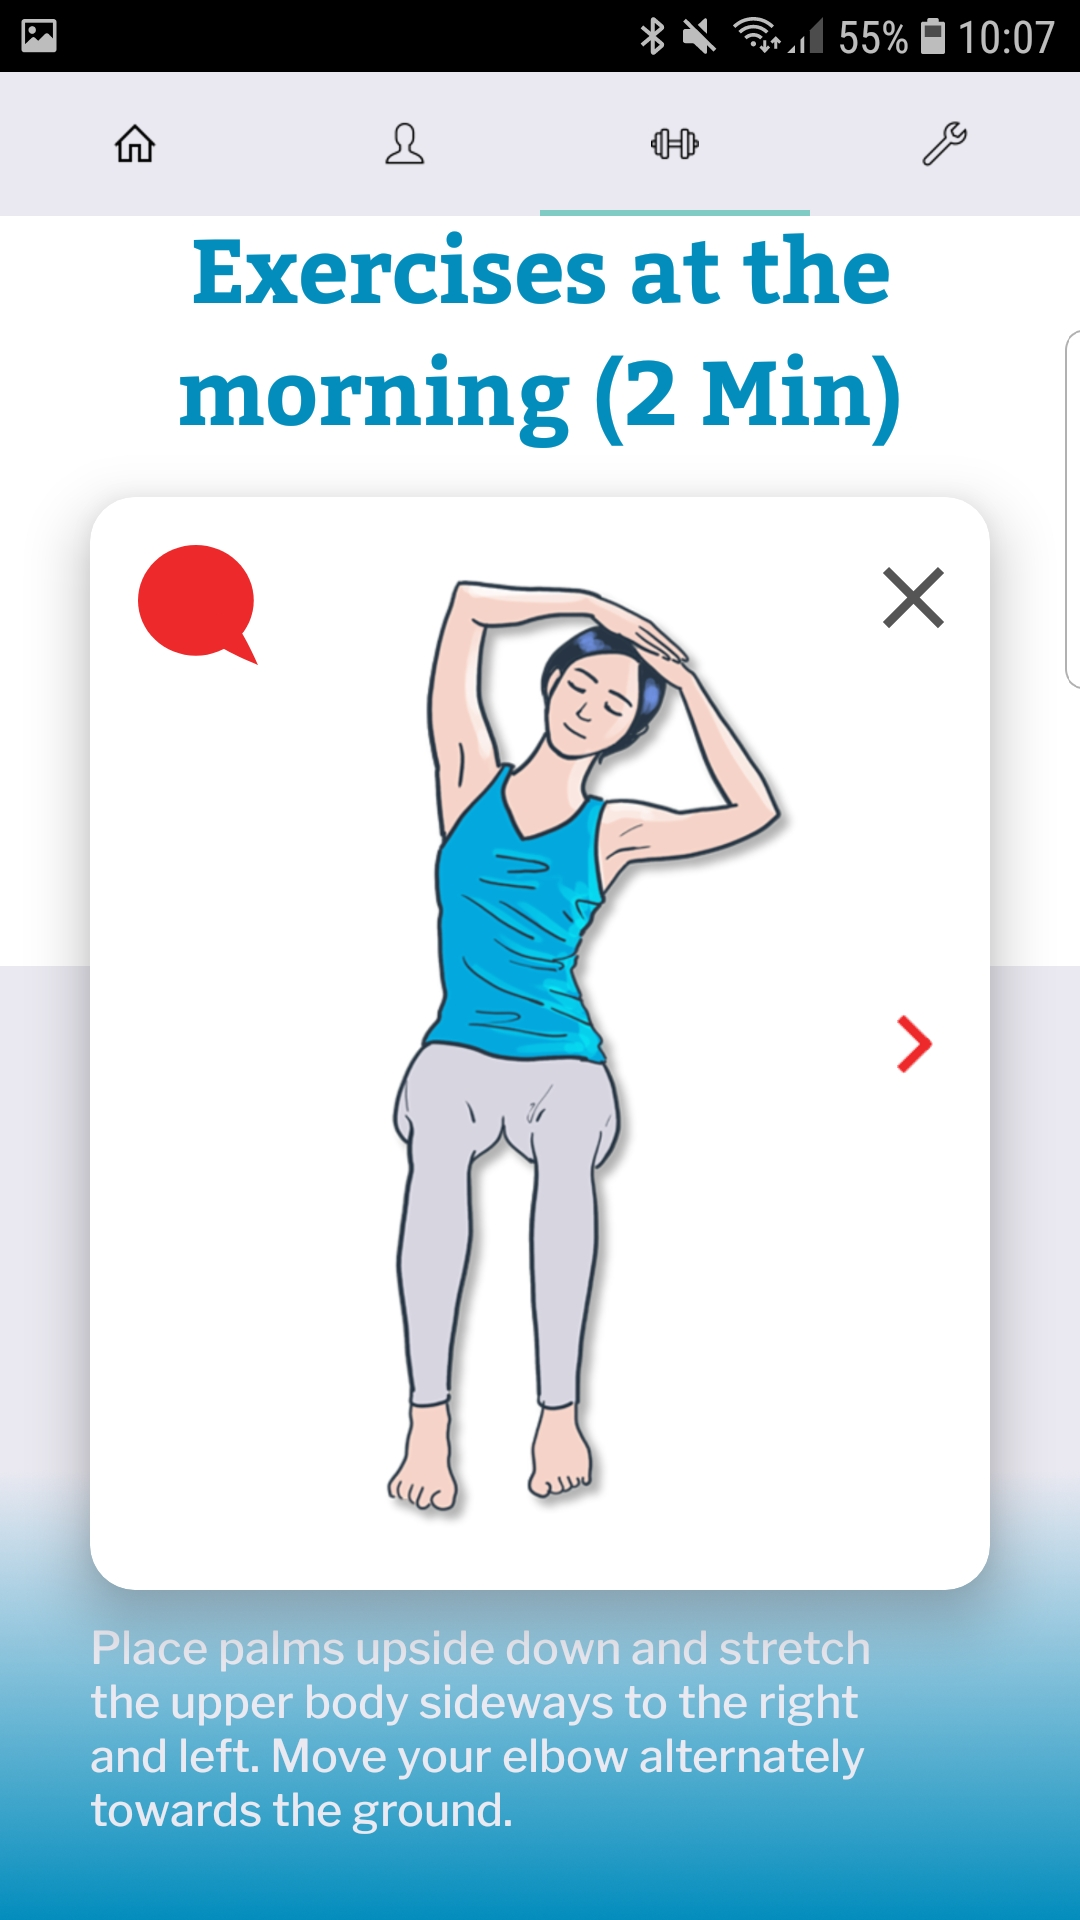
\includegraphics[width=0.5\textwidth]{excercise.jpg}
	\caption{\label{fig:Fitnesübung}Fitnessübungen zu einem bestimmten Schmerzbereich}
	
\end{figure}

\begin{figure}[ht]
	\centering
	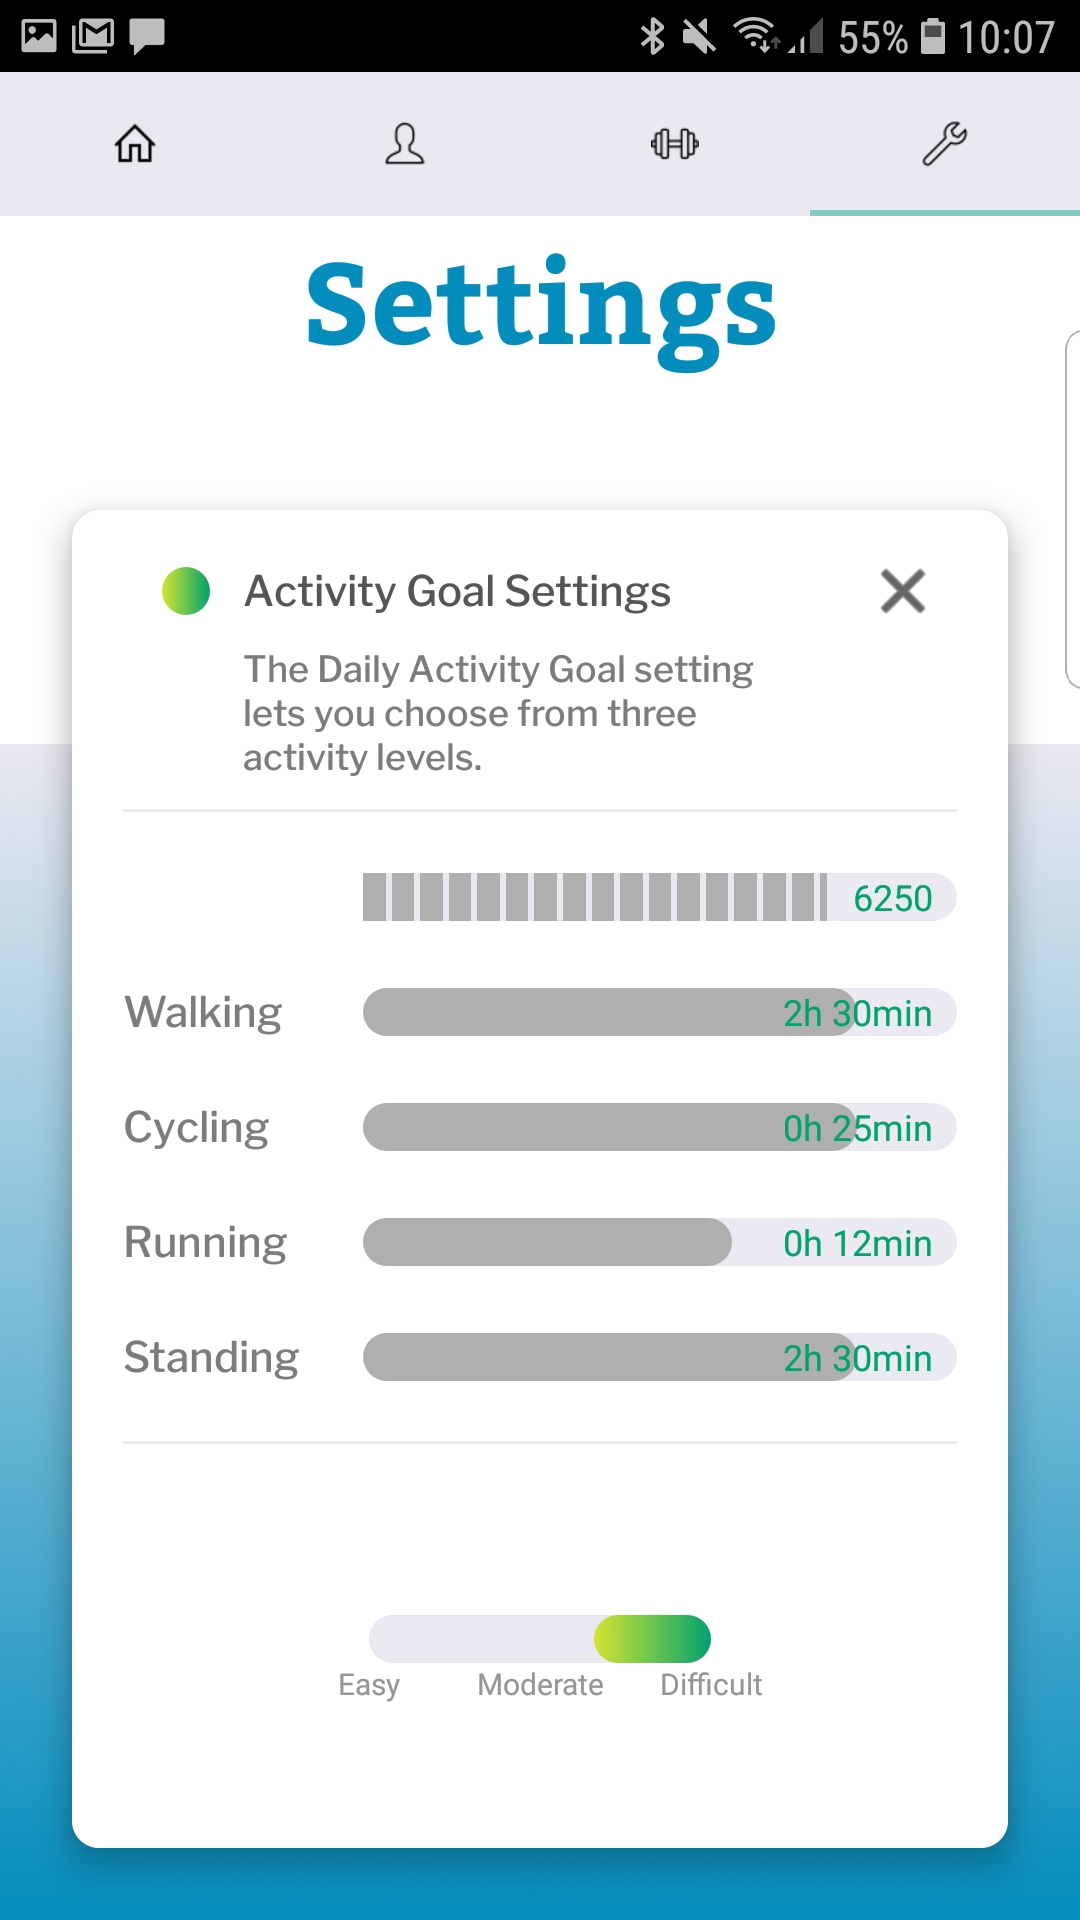
\includegraphics[width=0.5\textwidth]{settings.jpg}
	\caption{\label{fig:GoalSettings}Einstellung der Schwierigkeitslevels}
	
\end{figure}

